\chapter{Electromagnetic induction}

\section{Definitions}
\begin{marginfigure}
	\centering
	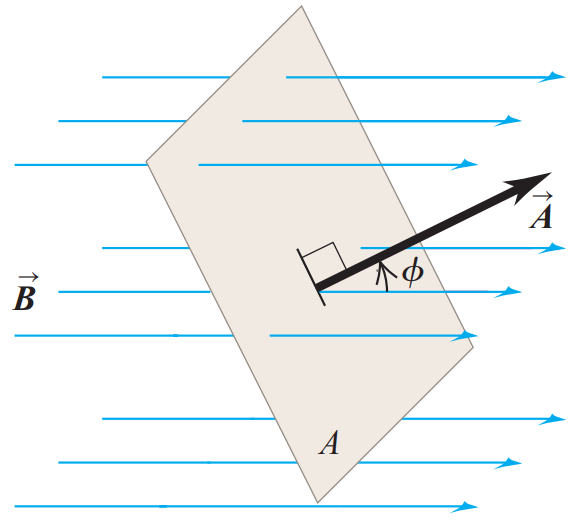
\includegraphics[width=.85\textwidth]{assets/phi-b.png}
	\caption{\(\Phi = B\cdot A\cos\phi = \ab(B\cos\phi) A\)}
	\label{fig:phi-b}
\end{marginfigure}
\begin{definition}{Magnetic flux}{bflux}
	The product of magnetic flux density \(B\) and cross-sectional area \(A_\perp\)
	\it{perpendicular} to the direction of \(B\). [weber: \unit{\weber}]
	\[\Phi = BA_\perp = B_\perp A\]
	\footnotesize
	\qty{1}{\weber} is the magnetic flux through a surface of area \qty{1}{\metre\squared} if a magnetic field
	of flux density \qty{1}{\tesla} is perpendicular to the surface.
\end{definition}

\begin{definition}{Magnetic flux linkage}{bflux-linkage}
	The product of the number of turns and the magnetic flux through each turn.
	\[\Phi_\text{link} = N\Phi\]
\end{definition}

\section{Faraday's law}
\begin{definition}{Faraday's law}{faraday}
	Magnitude of the induced emf \(\mathcal{E}\) is \it{directly proportional}
	to the rate of change of magnetic flux linkage \it{or the rate of cutting of magnetic flux}.
	\[\mathcal{E} = \ab|\odv{\Phi}{t}|\]
\end{definition}

\begin{marginfigure}
	\centering
	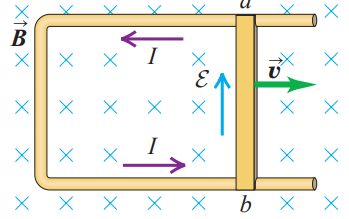
\includegraphics[width=\textwidth]{assets/u-loop.png}
	\caption{Sliding bar}
	\label{fig:u-loop}
\end{marginfigure}

\begin{example}{}{u-loop}
	(\Cref{fig:u-loop}) A conducting bar of length \(L\) slides on two parallel conducting rails in a uniform magnetic field
	\(B\) directed into the page. The bar moves to the right with a constant velocity \(v\). \it{What is the emf induced in the bar?}
	\\
	After a small time interval \(\odif{t}\), the bar moves a horizontal distance \(\odif{s}\).
	In this time, there will be a small change in magnetic flux, \(\odif{\Phi} = B\odif{A} = BL\odif{s}\).
	Since \(\epsilon \propto \odv{\Phi}{t}\),
	\begin{align*}
		\mathcal{E} & = \ab|\odv{\Phi}{t}| \\
		            & = B\ab|\odv{A}{t}|   \\
		            & = BL\ab|\odv{s}{t}|  \\
		            & = BLv
	\end{align*}
\end{example}

\begin{marginfigure}
	\centering
	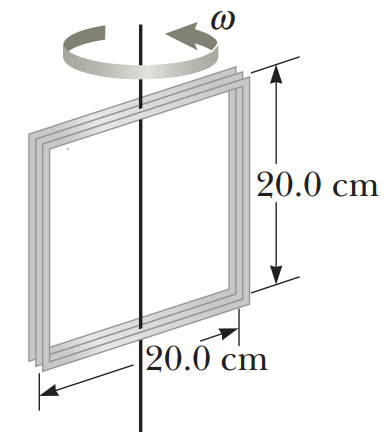
\includegraphics[width=.67\textwidth]{assets/rotating-coil.png}
	\caption{Rotating square loop}
	\label{fig:square-loop}
\end{marginfigure}
\begin{example}{}{rotating-loop}
	(\Cref{fig:square-loop}) A \(N\)-turn square loop of side \(x\) rotates in a uniform magnetic field \(B\)
	with an angular frequency \(\omega\). What is the \it{maximum emf} induced in the loop?
	\\\\
	At any time \(t\), the angle the loop makes with the magnetic field is \(\theta = \omega t\).
	Then the magnetic flux linkage is
	\begin{equation*}
		\Phi = NBA_\perp       = NBx^2\cos\theta  =NBx^2\cos\omega t
	\end{equation*}
	So the induced emf is
	\begin{align*}
		\mathcal{E}      & = \ab|\odv{\Phi}{t}|                \\
		                 & = NBx^2 \ab|\odv{}{t} \cos\omega t| \\
		                 & =  NB\omega x^2\sin\omega t         \\
		\max \mathcal{E} & = NB\omega x^2
	\end{align*}
\end{example}
\begin{marginfigure}
	\centering
	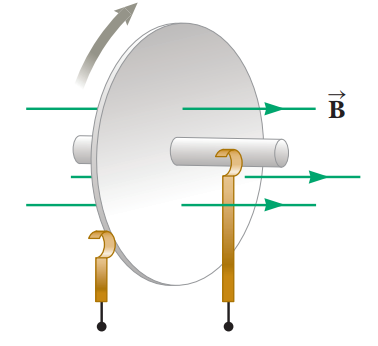
\includegraphics[width=.8\textwidth]{assets/faraday-disk.png}
	\label{fig:faraday-disk}
	\caption{Faraday disk}
\end{marginfigure}

\begin{example}{}{faraday-disk}
	(\Cref{fig:faraday-disk}) A uniform magnetic field \(B\) is passed
	through a rotating conducting disk of radius \(r\) and const.~angular velocity \(\omega\).
	What is the magnitude of the induced emf?

	For a short time \(\odif{t}\), the disk rotates through a small angle \(\odif{\theta} = \omega\odif{t}\) (by definition).
	The small area swept out by the disk in this time is \(\odif{A} = \f{1}{2}r^2\odif{\theta}\).
	Then
	\begin{align*}
		\mathcal{E} & = \ab|\odv{\Phi}{t}|       \\
		            & = B\ab|\odv{A}{t}|         \\
		            & = \f{1}{2}Br^2\dot{\theta} \\
		            & = \f{1}{2}Br^2\omega
	\end{align*}
\end{example}

\section{Lenz's law}
\begin{definition}{Lenz's law}{lenz}
	The polarity of the induced emf is such that the induced current
	creates a magnetic field to \it{oppose the change in magnetic flux}.
	\[\mathcal{E} = -\odv{\Phi}{t}\]
\end{definition}

How to determine \term{direction of induced current}:
\begin{enumerate}
	\item Pick a point of view.
	\item Determine the direction of the change in magnetic flux (increasing/decreasing?).
	\item Flip the direction to get the direction of the induced magnetic field (created by the induced current).
	\item Use RHGR to obtain the direction of the induced current. {\small Induced emf is in this direction too.}
\end{enumerate}

\begin{example}{}{u-loop-2}
	Referring to \cref{fig:u-loop}, what is the direction of induced current?
	\begin{itemize}
		\item As the bar moves \it{rightwards}, there is an increase in magnetic flux \it{rightwards}.
		\item By Lenz's law, increase in magnetic flux induces an emf to create a magnetic field \it{outwards}.
		\item Using RHGR, the direction of the induced current in the rectangular loop formed is \it{anticlockwise}.
	\end{itemize}
\end{example}
\begin{marginfigure}
	\centering
	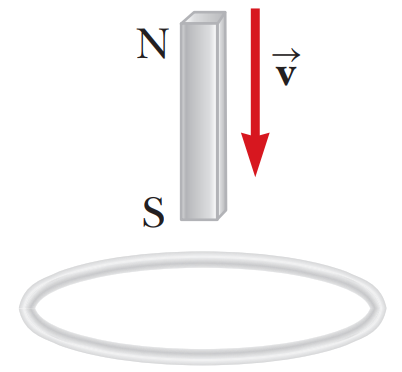
\includegraphics[width=.67\textwidth]{assets/falling-magnet.png}
	\caption{Falling magnet under gravity}
	\label{fig:falling-magnet}
\end{marginfigure}
\begin{example}{}{falling-magnet}
	Referring to \cref{fig:falling-magnet}, what is the direction of induced current?
	\vspace*{1em}
	When the magnet enters the loop,
	\begin{itemize}
		\item there is increasing upward flux (since \(\va{B}\) of bar magnet points upwards).
		\item By Lenz's law, the induced emf creates a magnetic field to oppose the flux change, so the \it{induced magnetic field is downwards}.
		\item By RHGR, \it{induced current is clockwise}.
	\end{itemize}
	As the magnet continues falling, the magnet accelerates (due to gravity).
	\begin{itemize}
		\item Upward magnetic flux continues to increase, since the velocity of the magnet increases.
		\item By Lenz's law, the induced emf creates a magnetic field to oppose the flux change, so the \it{induced magnetic field is downwards}.
		\item By RHGR, \it{induced current is clockwise}, and \it{of an increasing magnitude}.
		\item Induced emf \it{increases in magnitude}.
	\end{itemize}
	\vspace*{.5em}
	At the instant where the magnet leaves,
	\begin{itemize}
		\item there is a sudden decrease in upward magnetic flux.
		\item By Lenz's law, the induced emf creates a magnetic field to oppose the flux change, so the \it{induced magnetic field is upwards}.
		\item By RHGR, \it{induced current is anticlockwise}.
	\end{itemize}
\end{example}

\section{Eddy currents}
Eddy currents form when the magnetic flux varies periodically (e.g.~through an alternating current, or mechanical oscillation).
\begin{marginfigure}
	\centering
	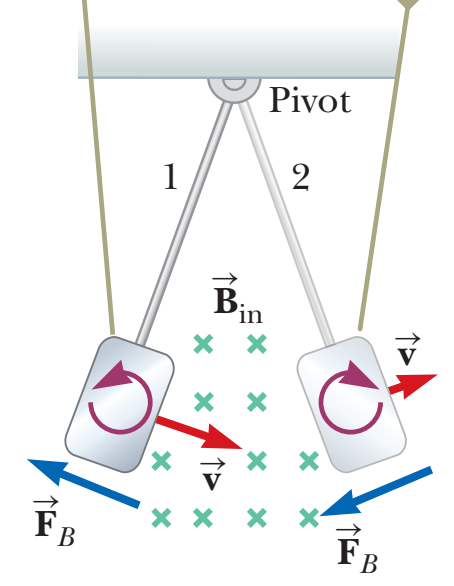
\includegraphics[width=.8\textwidth]{assets/eddy-current.png}
	\caption{Eddy currents}
	\label{fig:eddy-current}
\end{marginfigure}
We can \bf{reduce eddy currents} by laminating conducting components (building up in thin layers).
Increased resistance \(\implies\) reduced eddy currents \(\implies\) reduced energy loss due to eddy currents.

\section{Transformers}
\it{Ideal transformers} have coils of \it{zero resistance}.
\[\lf{V_s}{V_p} = \lf{N_s}{N_p}\]

\begin{marginfigure}
	\centering
	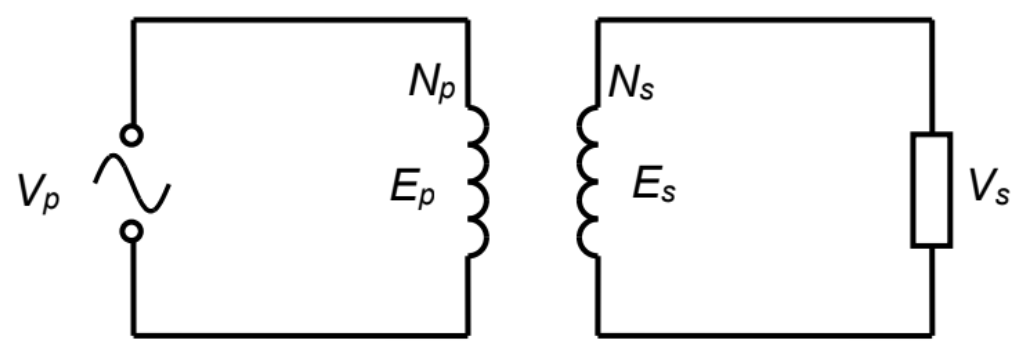
\includegraphics[width=\textwidth]{assets/transformer.png}
	\caption{Transformer}
	\label{fig:transformer}
\end{marginfigure}

In an ideal situation, the transformers are also \qty{100}{\percent} efficient:
\begin{align*}
	P_p     & = P_s     \\
	V_p I_p & = V_s I_s
\end{align*}
If the transformer is not ideal, then calculate \(P_\text{out}\) from \(P_\text{in}\)
given \(\eta\).

\hil{Eddy currents} can be reduced by \it{laminating the transformer core}
\(\implies\) increased resistance \(\implies\) reduced eddy currents \(\implies\) reduced
energy loss (thermal) \(\implies\) better efficiency.

\hil{Hysteresis} is energy loss resulting from direction of a.c.~periodically reversing.
It causes heating in the core. Hysteresis can be reduced by using \it{soft iron core}
or \it{alloys}.
